\documentclass[11pt,a4paper]{ivoa}
\input tthdefs

\usepackage[utf8]{inputenc}
\usepackage{tabularx}
\usepackage{mathtools}

\usepackage{listings}
\lstloadlanguages{XML,sh}
\lstset{flexiblecolumns=true,numberstyle=\small,numbers=left}

\usepackage{hyperref}

%\newcommand{\hfoot}[1] {\footnote{See URL: \href{#1} {{\tt #1}}   }}

\title{Astronomical Data Query Language}

\ivoagroup{Data Access Layer Working Group}

\author[http://wiki.ivoa.net/twiki/bin/view/IVOA/IvoaVOQL]{The IVOA Virtual Observatory Query Language (VOQL) working group members}
\author[http://wiki.ivoa.net/twiki/bin/view/IVOA/IvoaDAL]{The IVOA Data Access Layer (DAL) working group members}

\editor[http://wiki.ivoa.net/twiki/bin/view/IVOA/DaveMorris]{Dave Morris}

\previousversion[http://www.ivoa.net/Documents/ADQL/2.0]{ADQL-2.0}

\begin{document}

\begin{abstract}
This document describes the Astronomical Data Query Language (ADQL).
ADQL has been developed based on SQL92.
This document describes the subset of the SQL grammar supported by ADQL.
Special restrictions and extensions to SQL92 have been defined in order
to support generic and astronomy specific operations.
\end{abstract}

\section*{Acknowledgments}

The authors would like to acknowledge all contributors to this and previous 
versions of this standard, especially:
P. Dowler,
J. Lusted,
M. A. Nieto-Santisteban,
W. O'Mullane,
M. Ohishi,
I. Ortiz,
P. Osuna,
Y Shirasaki,
and
A. Szalay.

\section*{Conformance-related definitions}

The words ``MUST'', ``SHALL'', ``SHOULD'', ``MAY'', ``RECOMMENDED'', and
``OPTIONAL'' (in upper or lower case) used in this document are to be
interpreted as described in IETF standard, \citet{std:RFC2119}.

The \emph{Virtual Observatory (VO)} is a general term for a collection of
federated resources that can be used to conduct astronomical research,
education, and outreach. The \href{http://www.ivoa.net}{International Virtual
Observatory Alliance (IVOA)} is a global collaboration of separately funded
projects to develop standards and infrastructure that enable VO applications.

\clearpage
\section{Introduction}
\label{sec:introduction}

The Astronomical Data Query Language (ADQL) is the language used by the
International Virtual Observatory Alliance (IVOA) to represent astronomy
queries posted to VO services. The IVOA has developed several standardized
protocols to access astronomical data, e.g., SIAP and SSAP for image and
spectral data respectively. These protocols might be satisfied using a single
table query. However, different VO services have different needs in terms
of query complexity and ADQL arises in this context.

The ADQL specification makes no distinction between core and advanced or
extended functionalities. Hence ADQL has been built according to a single
Backus Naur Form (BNF) based language definition. Any service making use of ADQL would
then define the level of compliancy to the language. This would allow the
notion of core and extension to be service-driven and it would decouple the
language from the service specifications.

ADQL is based on the Structured Query Language (SQL), especially on SQL 92. The
VO has a number of tabular data sets and many of them are stored in relational
databases, making SQL a convenient access means. A subset of the SQL grammar
has been extended to support queries that are specific to astronomy. Similarly
to SQL, the ADQL language definition is not semantically safe by design and
therefore this specification defines syntactical correctness only. Type safety
has been achieved as far as it can be done in SQL. The exact meaning of keywords
indicating requirement levels can be found in the References section.
%Should this be 'Conformance-related definitions' not 'References' ?

\clearpage
\subsection{Role within the VO Architecture}
\label{sec:role}

\begin{figure}
\centering
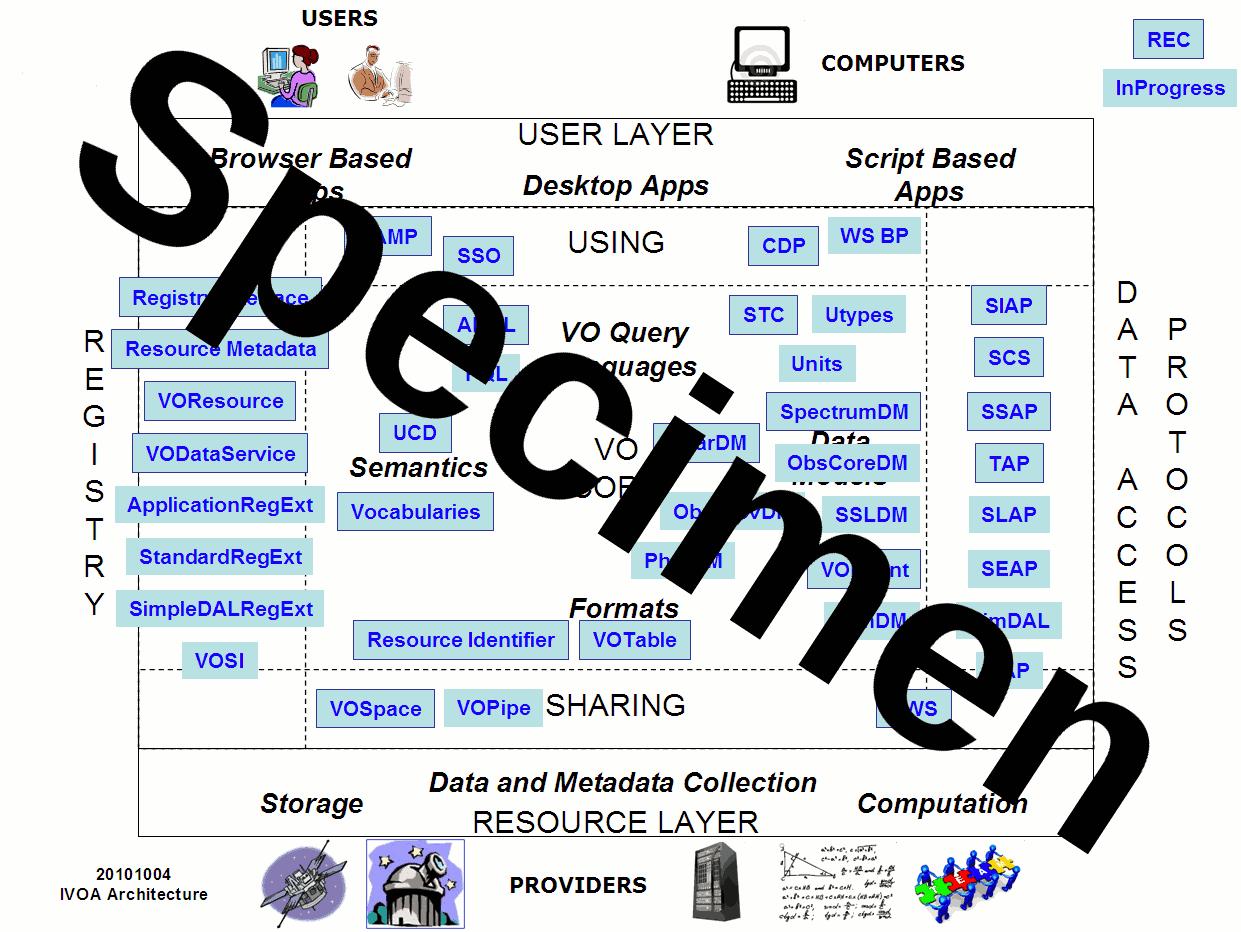
\includegraphics[width=0.9\textwidth]{archdiag.png}
\caption{Architecture diagram for this document}
\label{fig:archdiag}
\end{figure}

Fig.~\ref{fig:archdiag} shows the role this document plays within the
IVOA architecture \citep{note:VOARCH}.

\clearpage
\section{Astronomical Data Query Language (ADQL)}
\label{sec:language}

This section describes the ADQL language specification. We will define in
subsequent sections the syntax for the special characters, reserved and non-
reserved words, identifiers and literals and then, finally, the syntax for
the query expression.

The formal notation for syntax of computing languages is often expressed
in BNF. This syntax is used by popular tools for
producing parsers. Appendix A to this document provides the full BNF grammar
for ADQL. The following conventions are used through this document:

\begin{itemize}
    \item Optional items are enclosed in meta symbols \verb:[: and \verb:]:
    \item A group of items is enclosed in meta symbols \verb:{: and \verb:}:
    \item Repetitive item (zero or more times) are followed by \verb:...:
    \item Terminal symbols are enclosed by \verb:<: and \verb:>:
    \item Terminals of meta-symbol characters (\verb:=,[,],(,),<,>,*:) are surrounded by quotes (\verb:“:) to distinguish them from meta-symbols
    \item Case insensitiveness unless otherwise stated
\end{itemize}

\clearpage
\subsection{Characters, Keywords, Identifiers and Literals}
\subsubsection{Characters}
\label{sec:characters}

The language allows simple Latin letters (lower and upper case, i.e.
\verb:{aA-zZ}):, digits (\verb:{0-9}:) and the following special characters:

\begin{itemize}
    \item space
    \item single quote (\verb:’:)
    \item double quote (\verb:“:)
    \item percent (\verb:%:)
    \item left and right parenthesis
    \item asterisk (\verb:*:)
    \item plus sign (\verb:+:)
    \item minus sign (\verb:-:)
    \item comma (\verb:,:)
    \item period (\verb:.:)
    \item solidus (\verb:/:)
    \item colon (\verb.:.)
    \item semicolon (\verb:;:)
    \item less than operator (\verb:<:)
    \item equals operator (\verb:=:)
    \item greater than operator (\verb:>:)
    \item underscore (\verb:_:)
    \item ampersand (\verb:&:)
    \item question mark (\verb:?:)
    \item circumflex (\verb:^:)
    \item tilde (\verb:~:)
    \item vertical bar (\verb:|:)
\end{itemize}

\subsubsection{Keywords and Identifiers}
\label{sec:keywords}

Besides the character set, the language provides a list of reserved keywords
plus the syntax description for regular identifiers.

A reserved keyword has a special meaning in ADQL and cannot be used as
an identifier unless it is isolated using the ADQL escape syntax defined
in section \ref{sec:adql.escape}.

The AQDL specification extends the list of SQL92 reserved keywords to accommodate
those useful for astronomical purposes and/or present in a subset of vendor
specific languages only (e.g. \verb:TOP:).

Although the following lists are all in UPPERCASE, the matching of keywords
is case insensitive.

\subsubsection{SQL reserved keywords}
\label{sec:adql.keywords}

\noindent
\texttt{ABSOLUTE,} \texttt{ACTION,} \texttt{ADD,} \texttt{ALL,} 
\texttt{ALLOCATE,} \texttt{ALTER,} \texttt{AND,} \texttt{ANY,} 
\texttt{ARE,} \texttt{AS,} \texttt{ASC,} \texttt{ASSERTION,} 
\texttt{AT,} \texttt{AUTHORIZATION,} \texttt{AVG,} \texttt{BEGIN,} 
\texttt{BETWEEN,} \texttt{BIT,} \texttt{BIT\_LENGTH,} \texttt{BOTH,} 
\texttt{BY,} \texttt{CASCADE,} \texttt{CASCADED,} \texttt{CASE,} 
\texttt{CAST,} \texttt{CATALOG,} \texttt{CHAR,} \texttt{CHARACTER,} 
\texttt{CHARACTER\_LENGTH,} \texttt{CHAR\_LENGTH,} \texttt{CHECK,} 
\texttt{CLOSE,} \texttt{COALESCE,} \texttt{COLLATE,} 
\texttt{COLLATION,} \texttt{COLUMN,} \texttt{COMMIT,} 
\texttt{CONNECT,} \texttt{CONNECTION,} \texttt{CONSTRAINT,} 
\texttt{CONSTRAINTS,} \texttt{CONTINUE,} \texttt{CONVERT,} 
\texttt{CORRESPONDING,} \texttt{COUNT,} \texttt{CREATE,} 
\texttt{CROSS,} \texttt{CURRENT,} \texttt{CURRENT\_DATE,} 
\texttt{CURRENT\_TIME,} \texttt{CURRENT\_TIMESTAMP,} 
\texttt{CURRENT\_USER,} \texttt{CURSOR,} \texttt{DATE,} \texttt{DAY,} 
\texttt{DEALLOCATE,} \texttt{DECIMAL,} \texttt{DECLARE,} 
\texttt{DEFAULT,} \texttt{DEFERRABLE,} \texttt{DEFERRED,} 
\texttt{DELETE,} \texttt{DESC,} \texttt{DESCRIBE,} 
\texttt{DESCRIPTOR,} \texttt{DIAGNOSTICS,} \texttt{DISCONNECT,} 
\texttt{DISTINCT,} \texttt{DOMAIN,} \texttt{DOUBLE,} \texttt{DROP,} 
\texttt{ELSE,} \texttt{END,} \texttt{END-EXEC,} \texttt{ESCAPE,} 
\texttt{EXCEPT,} \texttt{EXCEPTION,} \texttt{EXEC,} \texttt{EXECUTE,} 
\texttt{EXISTS,} \texttt{EXTERNAL,} \texttt{EXTRACT,} \texttt{FALSE,} 
\texttt{FETCH,} \texttt{FIRST,} \texttt{FLOAT,} \texttt{FOR,} 
\texttt{FOREIGN,} \texttt{FOUND,} \texttt{FROM,} \texttt{FULL,} 
\texttt{GET,} \texttt{GLOBAL,} \texttt{GO,} \texttt{GOTO,} 
\texttt{GRANT,} \texttt{GROUP,} \texttt{HAVING,} \texttt{HOUR,} 
\texttt{IDENTITY,} \texttt{IMMEDIATE,} \texttt{IN,} 
\texttt{INDICATOR,} \texttt{INITIALLY,} \texttt{INNER,} 
\texttt{INPUT,} \texttt{INSENSITIVE,} \texttt{INSERT,} \texttt{INT,} 
\texttt{INTEGER,} \texttt{INTERSECT,} \texttt{INTERVAL,} 
\texttt{INTO,} \texttt{IS,} \texttt{ISOLATION,} \texttt{JOIN,} 
\texttt{KEY,} \texttt{LANGUAGE,} \texttt{LAST,} \texttt{LEADING,} 
\texttt{LEFT,} \texttt{LEVEL,} \texttt{LIKE,} \texttt{LOCAL,} 
\texttt{LOWER,} \texttt{MATCH,} \texttt{MAX,} \texttt{MIN,} 
\texttt{MINUTE,} \texttt{MODULE,} \texttt{MONTH,} \texttt{NAMES,} 
\texttt{NATIONAL,} \texttt{NATURAL,} \texttt{NCHAR,} \texttt{NEXT,} 
\texttt{NO,} \texttt{NOT,} \texttt{NULL,} \texttt{NULLIF,} 
\texttt{NUMERIC,} \texttt{OCTET\_LENGTH,} \texttt{OF,} \texttt{ON,} 
\texttt{ONLY,} \texttt{OPEN,} \texttt{OPTION,} \texttt{OR,} 
\texttt{ORDER,} \texttt{OUTER,} \texttt{OUTPUT,} \texttt{OVERLAPS,} 
\texttt{PAD,} \texttt{PARTIAL,} \texttt{POSITION,} 
\texttt{PRECISION,} \texttt{PREPARE,} \texttt{PRESERVE,} 
\texttt{PRIMARY,} \texttt{PRIOR,} \texttt{PRIVILEGES,} 
\texttt{PROCEDURE,} \texttt{PUBLIC,} \texttt{READ,} \texttt{REAL,} 
\texttt{REFERENCES,} \texttt{RELATIVE,} \texttt{RESTRICT,} 
\texttt{REVOKE,} \texttt{RIGHT,} \texttt{ROLLBACK,} \texttt{ROWS,} 
\texttt{SCHEMA,} \texttt{SCROLL,} \texttt{SECOND,} \texttt{SECTION,} 
\texttt{SELECT,} \texttt{SESSION,} \texttt{SESSION\_USER,} 
\texttt{SET,} \texttt{SIZE,} \texttt{SMALLINT,} \texttt{SOME,} 
\texttt{SPACE,} \texttt{SQL,} \texttt{SQLCODE,} \texttt{SQLERROR,} 
\texttt{SQLSTATE,} \texttt{SUBSTRING,} \texttt{SUM,} 
\texttt{SYSTEM\_USER,} \texttt{TABLE,} \texttt{TEMPORARY,} 
\texttt{THEN,} \texttt{TIME,} \texttt{TIMESTAMP,} 
\texttt{TIMEZONE\_HOUR,} \texttt{TIMEZONE\_MINUTE,} \texttt{TO,} 
\texttt{TRAILING,} \texttt{TRANSACTION,} \texttt{TRANSLATE,} 
\texttt{TRANSLATION,} \texttt{TRIM,} \texttt{TRUE,} \texttt{UNION,} 
\texttt{UNIQUE,} \texttt{UNKNOWN,} \texttt{UPDATE,} \texttt{UPPER,} 
\texttt{USAGE,} \texttt{USER,} \texttt{USING,} \texttt{VALUE,} 
\texttt{VALUES,} \texttt{VARCHAR,} \texttt{VARYING,} \texttt{VIEW,} 
\texttt{WHEN,} \texttt{WHENEVER,} \texttt{WHERE,} \texttt{WITH,} 
\texttt{WORK,} \texttt{WRITE,} \texttt{YEAR,} \texttt{ZONE} 

\subsubsection{ADQL reserved keywords}
\label{sec:adql.keywords}

\noindent
\texttt{ABS,} \texttt{ACOS,} \texttt{ASIN,} \texttt{ATAN,} 
\texttt{ATAN2,} \texttt{CEILING,} \texttt{COS,} \texttt{DEGREES,} 
\texttt{EXP,} \texttt{FLOOR,} \texttt{LOG,} \texttt{LOG10,} 
\texttt{MOD,} \texttt{PI,} \texttt{POWER,} \texttt{RADIANS,} 
\texttt{RAND,} \texttt{ROUND,} \texttt{SIN,} \texttt{SQRT,} 
\texttt{TAN,} \texttt{TOP,} \texttt{TRUNCATE}
\newline
\newline
\noindent
\texttt{AREA,} \texttt{BOX,} \texttt{CENTROID,} \texttt{CIRCLE,} 
\texttt{CONTAINS,} \texttt{COORD1,} \texttt{COORD2,} 
\texttt{COORDSYS,} \texttt{DISTANCE,} \texttt{INTERSECTS,} 
\texttt{POINT,} \texttt{POLYGON}

\subsubsection{ADQL deprecated keywords}
\label{sec:adql.depwords}

\noindent
\texttt{REGION}

\subsubsection{Identifiers}
\label{sec:adql.identifiers}

Identifiers MUST begin with a letter
\verb:{aA-zZ}:, subsequent characters MAY be letters, underscores or
digits \verb:{0-9}: as follows:

\begin{verbatim}
<Latin_letter>... [{ <digit> | <Latin_letter> | <underscore> | }...]
\end{verbatim}

\subsubsection{Escape syntax}
\label{sec:adql.escape}

To address reserved keyword and special character conflicts the ADQL language
provides a way to escape a non-compliant identifiers by using the double
quote character \verb:": as a delimiter.

For example, to use the reserved word \verb:size: as a column name
it must be isolated using double quotes.

\begin{itemize}
    \item \verb:size: -- Invalid column name
    \item \verb:"size": -- Valid column name
\end{itemize}

\subsubsection{Case sensitivity}
\label{sec:adql.case}

In addition to isolating keyword conflicts and and special characters,
the double quote escape syntax also denotes case sensitivity.

Without double quotes, the following identifiers are all equivalent:
\begin{verbatim}
    alpha == Alpha == ALPHA
\end{verbatim}

When escaped using double quotes, the same set of identifiers are not equivalent:
\begin{verbatim}
    "alpha" != "Alpha" != "ALPHA"
\end{verbatim}

\subsubsection{Literals}
\label{sec:literals}

Finally we define the syntax rules for the different data types: string,
numeric and boolean.

A string literal is a character expression delimited by single quotes.

\begin{verbatim}
    <character_string_literal> ::=
        <quote> [ <character_representation>... ] <quote>
\end{verbatim}

Literal numbers are expressed in BNF as follows:

\begin{verbatim}
    <signed_numeric_literal> ::= [<sign>] <unsigned_numeric_literal>

    <unsigned_numeric_literal> ::= 
        <exact_numeric_literal>
      | <approximate_numeric_literal>
      | <unsigned_hexadecimal>
              
    <exact_numeric_literal> ::=
        <unsigned_decimal> [<period> [<unsigned_decimal>]]
      | <period><unsigned_decimal>

    <approximate_numeric_literal> ::= <mantissa> E <exponent>

    <mantissa> ::= <exact_numeric_literal>

    <exponent> ::= <signed_decimal>

    <signed_decimal> ::= [<sign>] <unsigned_decimal>

    <unsigned_decimal> ::= <digit>...

    <digit> ::= 0 | 1  | 2 | 3 | 4 | 5 | 6 | 7 | 8 | 9
    
    <sign> ::= <plus_sign> | <minus_sign>
\end{verbatim}

Hexadecimal literals are expressed using the 'C' style notation, e.g. \verb:0xFF:,
defined in BNF as follows :
\begin{verbatim}
    <unsigned_hexadecimal> ::= 0x<hex_digit>...

    hex_digit ::= <digit> | a | b | c | d | e | f | A | B | C | D | E | F
\end{verbatim}

Hexadecimal literals are not case sensitive.

Hexadecimal literals can only be used to create integer data types, SMALLINT, INTEGER and BIGINT.

Boolean literals are expressed in BNF as follows:

\begin{verbatim}
    <boolean_literal> ::= True | False
\end{verbatim}

Boolean literals are not case sensitive.

Regarding the usage of other data types like datetime and timestamp, ADQL
can deal with them similarly to how SQL does: using the string literal
construct. As Relation Database Manager Systems (RDBMS) do, a service should
be able to implicitly convert strings to internal (datetime or timestamp)
form using a variety of techniques, where e.g. ISO 8601 is an acceptable
format. Therefore, as with other string representations, it should be up to
the service capability to understand such specific formats.

\clearpage
\subsection{Query syntax}
\label{sec:syntax}

A full and complete syntax of the select statement can be found in “Appendix
A: BNF Grammar” at the \verb:<query_specification>: construct. A simplified
syntax for the \verb:SELECT: statement follows, showing the main constructs for the query
specification:

\begin{verbatim}
    SELECT
        [ ALL | DISTINCT ]
        [ TOP unsigned_decimal ]
        {
             * |
             { value_expression [ [AS] column_name ] }, ...
         }
        FROM {
                {
                table_name [ [AS] identifier ] |
                ( SELECT ....) [ [AS] identifier ] |
                table_name [NATURAL]
                    [ INNER | { LEFT | RIGHT | FULL [OUTER] } ]
                    JOIN table_name
                    [ON search_condition | USING ( column_name,...) ]
                },
            ...
            }

        [ WHERE search_condition ]
        [ GROUP BY column_name, ... ]
        [ HAVING search_condition ]
        [ ORDER BY
            { column_name | unsigned_decimal } [ ASC | DESC],
            ...
            ]
        [ OFFSET unsigned_decimal ]
\end{verbatim}

The SELECT statement defines a query to some derived table(s) specified
in the FROM clause. As a result of this query, a subset of the table(s)
is returned.
The order of the rows MAY be arbitrary unless an ORDER BY clause is specified.
A TOP clause MAY be specified to limit the number of rows returned. 
An OFFSET clause MAY be specified to skip a number of rows at the start
of the results.
If OFFSET is used in combination with a TOP clause then OFFSET is applied
first, then the result set is limited by TOP (see \ref{sec:offset}). 

The order of the columns to return SHALL be the same as the
order specified in the selection list, or the order defined in the original
table if asterisk is specified. The selection list MAY include any numeric,
string or geometry value expression.
In the following sections some constructs requiring further description
are presented.

\subsubsection{Table subqueries and Joins}
\label{sec:subqueries}

Table subqueries are present and can be used by some existing predicates
within the search condition (IN and BETWEEN most likely) or as an artifact
of building derived tables. Among the different types of join, ADQL supports
INNER and OUTER (LEFT, RIGHT and FULL) joins. If none is specified, the
default is INNER. All of these can be NATURAL or not. The join condition
does not support embedded sub joins.

\subsubsection{Search condition}
\label{sec:search}

The search condition can be part of several other clauses: JOIN, HAVING and,
obviously, WHERE. Standard logical operators are present in its description
(AND, OR and NOT). Five different types of predicates are present in which
different types of reserved keywords or characters are used:

\begin{itemize}
    \item Standard comparison operators: \verb:=:, \verb:!=:, \verb:<>:, \verb:<:, \verb:>:, \verb:<=:, \verb:>=:
    \item \verb:BETWEEN:
    \item \verb:LIKE:
    \item \verb:NULL:
    \item \verb:EXISTS:
\end{itemize}

In addition, some service implementations may also support the optional
ILIKE case-insensitive string comparison operator, defined in section \ref{sec:string.functions.ilike}.

\begin{itemize}
    \item \verb:ILIKE:
\end{itemize}

\clearpage
\subsection{Mathematical and Trigonometrical Functions}
\label{sec:math.functions}

ADQL declares a list of reserved keywords (Section \ref{sec:keywords}) which include
the mathematical and trigonometrical function names. Their syntax,
usage and description are detailed in the following tables:

\begin{table}[thm]\footnotesize
    \begin{tabular}{|p{0.20\textwidth}|p{0.125\textwidth}|p{0.125\textwidth}|p{0.55\textwidth}|}
        \hline

        \hline
        \textbf{Name} &
        \textbf{Argument \newline data type} &
        \textbf{Return \newline data type} &
        \textbf{Description}
        \tabularnewline

        \hline
        abs(x) &
        double&double &
        Returns the absolute value of x.
        \tabularnewline

        \hline
        ceiling(x) &
        double&double &
        Returns the smallest double value that is not less than the argument x and is equal to a mathematical integer.
        \tabularnewline

        \hline
        degrees(x) &
        double &
        double &
        Converts an angle to degrees. Argument x must be in radians.
        \tabularnewline

        \hline
        exp(x) &
        double &
        double &
        Returns Euler’s number e raised to the power of x.
        \tabularnewline

        \hline
        floor(x) &
        double &
        double &
        Returns the largest double value that is not greater than the argument x and is equal to a mathematical integer.
        \tabularnewline

        \hline
        log(x) &
        double &
        double &
        Returns the natural logarithm (base e) of a double value. Value x must be greater than zero.
        \tabularnewline

        \hline
        log10(x) &
        double &
        double &
        Returns the base 10 logarithm of a double value. Value x must be greater than zero.
        \tabularnewline

        \hline
        mod(x, y) &
        double &
        double &
        Returns the remainder of x/y.
        \tabularnewline
        
        \hline
        pi() &
        n/a &
        double &
        The \(\pi\) constant.
        \tabularnewline
        
        \hline
        power(x, y) &
        x double \newline y double &
        double &
        Returns the value of the first argument raised to the power of the second argument.
        \tabularnewline

        \hline
        radians(x) &
        double &
        double &
        Converts an angle to radians. Argument x must be in degrees.
        \tabularnewline

        \hline
        sqrt(x) &
        double &
        double &
        Returns the positive square root of a double value.
        \tabularnewline

        \hline
        rand(x) &
        integer &
        double &
        Returns a random value between 0.0 and 1.0, where x is a seed  value.
        \tabularnewline

        \hline
        round(x, n) &
        x double \newline n integer &
        double &
        Rounds double value x to n number of decimal places, with the default being to round to the nearest integer.
        To round to the left of the decimal point, a negative number should be provided.
        \tabularnewline

        \hline
        truncate(x, n) &
        x double \newline n integer &
        double &
        Returns the result of truncating the argument x to n decimal places.
        \tabularnewline

        \hline
    \end{tabular}
    \caption{Mathematical functions}
    \label{table:math.functions.table}
\end{table}

\begin{table}[thm]\footnotesize
    \begin{tabular}{|p{0.20\textwidth}|p{0.125\textwidth}|p{0.125\textwidth}|p{0.55\textwidth}|}
        \hline

        \hline
        \textbf{Name} &
        \textbf{Argument \newline data type} &
        \textbf{Return \newline data type} &
        \textbf{Description}
        \tabularnewline

        \hline
        acos(x) &
        double &
        double &
        Returns the arc cosine of an angle, in the range of 0 through \(\pi\) radians. Absolute value of x must be lower or equal than 1.0.
        \tabularnewline

        \hline
        asin(x) &
        double &
        double &
        Returns the arc sine of an angle, in the range of -\(\pi\)/2 through \(\pi\)/2 radians. Absolute value of x must be and lower or equal than 1.0.
        \tabularnewline

        \hline
        atan(x) &
        double &
        double &
        Returns the arc tangent of an angle, in the range of -\(\pi\)/2 through \(\pi\)/2 radians.
        \tabularnewline
        
        \hline
        atan2(y,x) &
        double &
        double &
        Converts rectangular coordinates x,y to polar angle. It computes the arc tangent of y/x in the range of –\(\pi\) through \(\pi\) radians.
        \tabularnewline

        \hline
        cos(x) &
        double &
        double &
        Returns the cosine of an angle, in the range of -1.0 through 1.0. Argument x must be in radians.
        \tabularnewline

        \hline
        sin(x) &
        double &
        double &
        Returns the sine of an angle, in the range of -1.0 through 1.0. Argument x must be in radians.
        \tabularnewline

        \hline
        tan(x) &
        double &
        double &
        Returns the tangent of an angle. Argument x must be in radians.
        \tabularnewline

        \hline
    \end{tabular}
    \caption{Trigonometrical functions}
    \label{table:trig.functions.table}
\end{table}

\clearpage
\section{ADQL Type System}
\label{sec:types}

ADQL defines no data definition language (DDL).
It is assumed that table definition and data ingestion are performed in
the underlying database's native language and type system.

However, column metadata needs to give column types in order to allow the
construction of queries that are both syntactically and semantically correct.
Examples of such metadata includes VODataService's \verb:TAPType:
(VODataService-1.1, \citet{std:VODS11}) or TAP's \verb:TAP_SCHEMA: (TAP-1.0, \citet{std:TAP}).

Services SHOULD, if at all possible, try to express their column metadata in
these terms even if the underlying database employs different types.
Services SHOULD also use the following mapping when interfacing to user data,
either by serializing result sets into VOTables or by ingesting user-provided
VOTables into ADQL-visible tables.
Where non-ADQL types are employed in the underlying database, implementors
SHOULD make sure that all operations that are possible with the recommended
ADQL type are also possible with the type used in the backend engine.
For instance, the ADQL string concatenation operator \verb:||: should be
applicable to all columns resulting from VOTable char-typed columns.

\begin{table}[thm]\footnotesize
    \begin{tabular}{|p{0.15\textwidth}|p{0.15\textwidth}|p{0.25\textwidth}|p{0.30\textwidth}|}
        \hline

        \hline
        \multicolumn{3}{|c|}{\textbf{VOTable}} &
        \multicolumn{1}{|c|}{\textbf{ADQL}}
        \tabularnewline
        
        \hline
        \textbf{datatype} &
        \textbf{arraysize} &
        \textbf{xtype} &
        \textbf{type}
        \tabularnewline

        \hline
        boolean &
        1 &
        - &
        BOOLEAN
        \tabularnewline

        \hline
        short &
        1 &
        - &
        SMALLINT
        \tabularnewline

        \hline
        int &
        1 &
        - &
        INTEGER
        \tabularnewline

        \hline
        long &
        1 &
        - &
        BIGINT
        \tabularnewline

        \hline
        float &
        1 &
        - &
        REAL
        \tabularnewline

        \hline
        double &
        1 &
        - &
        DOUBLE
        \tabularnewline

        \hline
        (numeric) &
        > 1 &
        - &
        implementation defined
        \tabularnewline

        \hline
        char &
        1 &
        - &
        CHAR(1)
        \tabularnewline

        \hline
        char &
        n &
        - &
        CHAR(n)
        \tabularnewline

        \hline
        char &
        n* &
        - &
        VARCHAR(n)
        \tabularnewline

        \hline
        unsignedByte &
        n &
        - &
        BINARY(n)
        \tabularnewline

        \hline
        unsignedByte &
        n* &
        - &
        VARBINARY(n)
        \tabularnewline

        \hline
        unsignedByte &
        n, *, n* &
        adql:BLOB &
        BLOB
        \tabularnewline

        \hline
        char &
        n, *, n* &
        adql:CLOB &
        CLOB
        \tabularnewline

        \hline
        char &
        n, *, n* &
        adql:TIMESTAMP &
        TIMESTAMP
        \tabularnewline

        \hline
        char &
        n, *, n* &
        adql:POINT &
        POINT
        \tabularnewline

        \hline
        char &
        n, *, n* &
        adql:REGION &
        REGION
        \tabularnewline

        \hline
    \end{tabular}
    \caption{VOTable/ADQL type mapping}
    \label{table:adql.votable.type.map}
\end{table}

\textit{"Implementation defined"} in the above table means that an
implementation is free to reject attempts to (de-)serialize values in
these types.
They are to be considered unsupported by ADQL, and the language provides
no means to manipulate \textit{"native"} representations of them.

References to REGION-typed columns must be valid wherever the ADQL
\textit{region} nonterminal is allowed. References to POINT-typed columns
must be valid wherever the ADQL \textit{point} nonterminal is allowed.

Comparing the equality of a boolean value or expression with another
boolean returns a boolean result.

When comparing the size of a boolean with another boolean, the value
True is greater than the value False.

Unless explicitly stated, the result of any other operation on boolean
values is undefined.

\clearpage
\section{Optional components}
\label{sec:optional}

In addition to the core components, the ADQL language also includes support
for optional features and functions.

The following sections define the optional features that are part of the
the ADQL language, but are not required in order to meet the standard for
a basic ADQL service.

It is up to each service implementation to declare which optional or
additional features it supports.

If a service does not declare support for an optional or additional feature,
then a client SHOULD NOT assume that the service supports that feature,
and SHOULD NOT make use of that feature in any ADQL queries that it sends.

\subsection{Service capabilities}
\label{sec:capabilities}

The TAPRegExt-1.0 standard \citep{std:TAPREGEXT} defines an XML schema that a service SHOULD
use to declare which optional or additional features it supports.

In general, each group of langauge features is identified by a \verb:type:
URI, and each individual feature within the group is identified by the
feature name.

Appendix \ref{sec:features} contains examples of how to declare support
for each of the langauge features defined in this document using the
TAPRegExt XML schema.

For full details on the XML schema and how it can be used, please refer to
the TAPRegExt \citep{std:TAPREGEXT} standard.

\subsection{Geometrical Functions}
\label{sec:geom.functions}
\subsubsection{Overview}
\label{sec:geom.functions.overview}

In addition to the mathematical functions, ADQL provides a set of geometrical
functions to enhance the astronomical usage of the language.

\begin{itemize}
    \item AREA
    \item BOX
    \item CENTROID
    \item CIRCLE
    \item CONTAINS
    \item COORD1
    \item COORD2
    \item COORDSYS
    \item DISTANCE
    \item INTERSECTS
    \item POINT
    \item POLYGON
    \item REGION
\end{itemize}

Special attention has to be paid to the REGION function. As can be seen more
in detail in Section \ref{sec:geom.functions.region}, this construct is a general purpose function and
it takes a string value expression as argument. The format of the string is
to be specified by a service that accepts ADQL by referring to a standard
format. Currently STC/s is the only standardized string
representation a service can declare.
% STC-reference 'Currently  STC/s (See [3] and [4])'

As can also be seen in the following sections, all these functions
have arguments being a geometrical, a string and/or a numerical value
expression. When these values represent spherical coordinates the units MUST
be in degrees (square degrees for area). If the cartesian coordinate system
is used, the vector coordinates MUST be normalized.

Regarding the legal ranges, for spherical coordinates, these SHOULD be [0, 360]
and [-90, 90]. In a cartesian coordinate system, there are no inherent limits
apart from the already mentioned constraint that vectors should be normalized. It remains
up to the service making use of ADQL to define the errors that should be raised
when using values outside these ranges.

For historical reasons, the geometry constructors (BOX, CIRCLE, POINT,
POLYGON) require a string-valued first argument. It was intended to carry
information on a reference system or other coordinate system metadata.
As of this version of the specification (2.1), this parameter has been
marked as deprecated. Services are permitted to ignore this parameter and
clients are advised to pass an empty string here. Future versions of this
specification may remove this parameter from the listed functions.

Generally speaking, all these geometrical functions cover three different
topics: data types, predicates and utility calculations. Each of these are
covered below.

\subsubsection{Data Type Functions}
\label{sec:geom.functions.type}

Certain functions represent geometry data types. These data types are BOX,
CENTROID, CIRCLE, POINT and POLYGON together with the generalized REGION data
type. The functions are similarly named and return a variable length binary
value. The semantics of these data types are based on the corresponding
concepts from the STC data model.
% STC-reference 'STC data model (See [3])'

Geometry data types are centered around the BNF construct
\verb:<value_expression>: which is central to data types within SQL.

\begin{verbatim}
    <value_expression> ::=
        <numeric_value_expression>
      | <string_value_expression>
      | <boolean_value_expression>
      | <geometry_value_expression>
\end{verbatim}

A \verb:<geometry_value_expression>: does not simply cover data type functions
(POINT, CIRCLE etc) but must also allow for user defined functions and
column values where a geometry data type is stored in a column.

Therefore, \verb:<geometry_value_expression>: is expanded as:

\begin{verbatim}
    <geometry_value_expression> ::= 
        <value_expression_primary>
      | <geometry_value_function>
\end{verbatim}

, where

\begin{verbatim}
    <geometry_value_function> ::=
        <box>
      | <centroid>
      | <circle>
      | <point>
      | <polygon>
      | <region>
      | <user_defined_function>
\end{verbatim}

and \verb:<value_expression_primary>: makes possible to use a column reference.

\subsubsection{Predicate Functions}
\label{sec:geom.functions.predicate}

Functions CONTAINS and INTERSECTS each accept two geometry data types
and return 1 or 0 according to whether the relevant verb (e.g.: "contains") is
satisfied against the two input geometries; 1 represents true and 0 represents
false. Each of these functions can be assembled into a predicate:

\begin{verbatim}
    SELECT * FROM SDSS as s WHERE CONTAINS(POINT(...), CIRCLE(...)) = 1
\end{verbatim}

, where the ... would represent the constituent parts of a CIRCLE and POINT
geometry.

One would expect later additions to ADQL to add to this range of functions. For
example: equals, disjoint, touches, crosses, within, overlaps and relate
are possibilities.

\subsubsection{Utility Functions}
\label{sec:geom.functions.utility}

Function COORDSYS extracts the coordinate system string from a given
geometry. To do so it accepts a geometry expression and returns a calculated
string value.

This function has been included as a string value function because it
returns a simple string value. Hence:

\begin{verbatim}
    <string_value_function> :: =
        <string_geometry_function> | <user_defined_function>

    <string_geometry_function> ::= <extract_coordsys>

    <extract_coordsys> ::=
        COORDSYS <left_paren> <geometry_value_expression> <right_paren>
\end{verbatim}

Note - as of this version of the specification (2.1), the COORDSYS function has
been marked as deprecated. This function may be removed in future versions
of this specification.

Functions like AREA, COORD1, COORD2 and DISTANCE accept a geometry and
return a calculated numeric value.

The specification defines two versions of the DISTANCE function,
one that accepts accept two geometries, and one that accepts four
separate numeric values, both forms return a numeric value.

The Predicate and most of the Utility functions have been included as numeric
value functions because they return simple numeric values. Thus:

\begin{verbatim}
    <numeric_value_function> ::=
        <trig_function>
      | <math_function>
      | <numeric_geometry_function>
      | <user_defined_function>
\end{verbatim}

where

\begin{verbatim}
    <numeric_geometry_function> ::=
        <predicate_geometry_function>
      | <non_predicate_geometry_function>
\end{verbatim}

and

\begin{verbatim}
    <non_predicate_geometry_function> ::=
        AREA <left_paren> <geometry_value_expression> <right_paren>
      | COORD1 <left_paren> <coord_value> <right_paren>
      | COORD2 <left_paren> <coord_value> <right_paren>
      | DISTANCE <left_paren>
            <coord_value> <comma>
            <coord_value>
            <right_paren>
      | DISTANCE <left_paren>
            <numeric_value_expression> <comma>
            <numeric_value_expression> <comma>
            <numeric_value_expression> <comma>
            <numeric_value_expression>
            <right_paren>
\end{verbatim}

and

\begin{verbatim}
    <predicate_geometry_function> ::= <contains> | <intersects>
\end{verbatim}

%\subsubsection{Function definitions}
\clearpage
\label{sec:geom.functions.definitions}

The following sections provide a detailed description for each geometrical
function. In each case, the functionality and usage is described rather
than going into the BNF grammar details as above.

\subsubsection{AREA}
\label{sec:geom.functions.area}
{\footnotesize Language feature :}\\
{\footnotesize \verb|type: ivo://ivoa.net/std/TAPRegExt#features-adql-geo|}\\
{\footnotesize \verb|name: AREA|}\\

This function computes the area, in square degrees, of a given geometry.

For example, the area of a circle of one degree radius centered on a position
of (25.4, -20.0) degrees would be written as follows:

\begin{verbatim}
    AREA(CIRCLE(‘’, 25.4, -20.0, 1))
\end{verbatim}

The coordinates of the circle center could also be directly derived from
either a POINT function (See \ref{sec:geom.functions.point}) or
the coordinate’s column references:

\begin{verbatim}
    AREA(CIRCLE(‘’, t.ra, t.dec, 1))
\end{verbatim}

, where \textit{t} would be the table and \textit{ra}, \textit{dec} the
column references for the circle center.

Inappropriate geometries for this construct (e.g. POINT) SHOULD either return
zero or throw an error message, the later to be defined by the service making
use of ADQL.

\subsubsection{BOX}
\label{sec:geom.functions.box}
{\footnotesize Language feature :}\\
{\footnotesize \verb|type: ivo://ivoa.net/std/TAPRegExt#features-adql-geo|}\\
{\footnotesize \verb|name: BOX|}\\

This function expresses a box on the sky. A box is a special case of Polygon,
defined purely for convenience, and it corresponds semantically to the STC Box
region. It is specified by a center position and size
% STC-reference 'region ([3], Section 4.5.1.5)'
(in both coordinates) defining a cross centered on the center position and
with arms extending, parallel to the coordinate axes at the center position,
for half the respective sizes on either side. The box’s sides are line
segments or great circles intersecting the arms of the cross in its end
points at right angles with the arms.

The function arguments specify the coordinate system, the center position
and both the width and height (arms) values, where:

\begin{itemize}
    \item the coordinate system is a string value expression as defined in Section \ref{sec:geom.functions.overview}.
    \item the center position is a comma separated numeric duple, with units and legal ranges as defined in Section \ref{sec:geom.functions.overview}.
    \item and the arms are numeric value expressions in degrees.
\end{itemize}

For example, a function expressing a box of ten degrees centered on a position
(25.4, -20.0) in degrees would be written as follows:

\begin{verbatim}
    BOX(‘’, 25.4, -20.0, 10, 10)
\end{verbatim}

As another example, the coordinates of the center position could also be
extracted from either a POINT function (See \ref{sec:geom.functions.point})
or the coordinate’s column references:

\begin{verbatim}
    BOX(‘’, t.ra, t.dec, 10, 10)
\end{verbatim}

, where \textit{t} would be the table and \textit{ra}, \textit{dec} the
column references for the center position.

To see what this function would return when listed in the select clause,
see Section \ref{sec:geom.select}.

\subsubsection{CENTROID}
\label{sec:geom.functions.centroid}
{\footnotesize Language feature :}\\
{\footnotesize \verb|type: ivo://ivoa.net/std/TAPRegExt#features-adql-geo|}\\
{\footnotesize \verb|name: CENTROID|}\\

This function computes the centroid of a given geometry and returns a POINT.

For example, the centroid of a circle of one degree radius centered in a
position of (25.4, -20.0) degrees would be written as follows :

\begin{verbatim}
    CENTROID(CIRCLE (‘’, 25.4, -20.0, 1))
\end{verbatim}

\subsubsection{CIRCLE}
\label{sec:geom.functions.circle}
{\footnotesize Language feature :}\\
{\footnotesize \verb|type: ivo://ivoa.net/std/TAPRegExt#features-adql-geo|}\\
{\footnotesize \verb|name: CIRCLE|}\\

This function expresses a circular region on the sky (a cone in space) and
corresponds semantically to the STC Circle region. The
function arguments specify the coordinate system, the center position,
and the radius, where:
% STC-reference STC Circle region ([3], Section 4.5.1.2)

\begin{itemize}
    \item the coordinate system is a string value expression as defined in Section \ref{sec:geom.functions.overview}.
    \item the center position is a comma separated numeric duple, with units and legal ranges as defined in Section \ref{sec:geom.functions.overview}.
    \item and the radius is a numeric value expression in degrees.
\end{itemize}

For example, a function expressing a circle of one degree radius centered on a
position of (25.4, -20.0) degrees would be written as follows:

\begin{verbatim}
    CIRCLE(‘’, 25.4, -20.0, 1)
\end{verbatim}

The coordinates of the center position could also be derived from either a
POINT function (See \ref{sec:geom.functions.point}) or the coordinate’s column references:

\begin{verbatim}
    CIRCLE(‘’, t.ra, t.dec, 1)
\end{verbatim}

, where \textit{t} would be the table and \textit{ra}, \textit{dec} the
column references for the center position.

To see what this function would return when listed in the select clause, see
Section \ref{sec:geom.select}.

\subsubsection{CONTAINS}
\label{sec:geom.functions.contains}
{\footnotesize Language feature :}\\
{\footnotesize \verb|type: ivo://ivoa.net/std/TAPRegExt#features-adql-geo|}\\
{\footnotesize \verb|name: CONTAINS|}\\

This numeric function determines if a geometry is wholly contained within
another. This is most commonly used to express the "point-in-shape" condition.

For example, to determine if a point with right ascension of 25 degrees
and declination of -19.5 degrees is within a circle of one degree radius
centered in a position of (25.4, -20.0) degrees and defined according to the
same coordinate system, we would make use of the CONTAINS function as follows:

\begin{verbatim}
    CONTAINS(
        POINT(‘’, 25.0,-19.5),
        CIRCLE(‘’, 25.4, -20.0, 1)
        )
\end{verbatim}

, where the CONTAINS function returns 1 (true) if the first argument is in
or on the boundary of the circle and 0 (false) otherwise. Thus, contains is
not symmetric in the meaning of the arguments. When used in the WHERE clause
of a query, the value must be compared to 0 or 1 to form an SQL predicate:

\begin{verbatim}
    CONTAINS(
        POINT(‘’, 25.0,-19.5),
        CIRCLE(‘’, 25.4, -20.0, 1)
        ) = 1
\end{verbatim}

for "does contain" and

\begin{verbatim}
    CONTAINS(
        POINT(‘’, 25.0,-19.5),
        CIRCLE(‘’, 25.4, -20.0, 1)
        ) = 0
\end{verbatim}

for "does not contain".

The arguments to the CONTAINS function can be (literal) values created
from the geometry types or they can be single column names or aliases (for
geometry stored in a database table). Since the two argument geometries may
be expressed in different coordinate systems, the function is responsible
for converting one (or both). If it cannot do so, it SHOULD throw an error
message, to be defined by the service making use of ADQL.

\subsubsection{COORD1}
\label{sec:geom.functions.coord1}
{\footnotesize Language feature :}\\
{\footnotesize \verb|type: ivo://ivoa.net/std/TAPRegExt#features-adql-geo|}\\
{\footnotesize \verb|name: COORD1|}\\

This function extracts the first coordinate value, in degrees, of a given
POINT (See \ref{sec:geom.functions.point}) or column reference.

For example, the right ascension of a point with position (25, -19.5) in
degrees would be obtained using the following expression:

\begin{verbatim}
    COORD1(POINT(‘’, 25.0,-19.5))
\end{verbatim}

, being the result a numeric value of 25.0 degrees. The first coordinate
could also be derived directly from a column reference as follows:

\begin{verbatim}
    COORD1(t.point)
\end{verbatim}
    
, where \textit{t} is the table and \textit{point} the column reference for
the POINT geometry stored in the database table.

\subsubsection{COORD2}
\label{sec:geom.functions.coord2}
{\footnotesize Language feature :}\\
{\footnotesize \verb|type: ivo://ivoa.net/std/TAPRegExt#features-adql-geo|}\\
{\footnotesize \verb|name: COORD2|}\\

This function extracts the second coordinate value, in degrees, of a given
POINT (See \ref{sec:geom.functions.point}) or column reference.

For example, the declination of a point with position (25, -19.5) in degrees,
would be obtained using the following expression:

\begin{verbatim}
    COORD2(POINT(‘’, 25.0,-19.5))
\end{verbatim}

, being the result a numeric value of -19.5 degrees. The second coordinate
could also be derived directly from a column reference as follows:

\begin{verbatim}
    COORD2(t.point)
\end{verbatim}

, where \textit{t} is the table and \textit{point} the column reference for
the POINT geometry stored in the database table.

\subsubsection{COORDSYS}
\label{sec:geom.functions.coordsys}
{\footnotesize Language feature :}\\
{\footnotesize \verb|type: ivo://ivoa.net/std/TAPRegExt#features-adql-geo|}\\
{\footnotesize \verb|name: COORDSYS|}\\

Note - as of this version of the specification (2.1), the COORDSYS function has
been marked as deprecated. This function may be removed in future versions
of this specification.

This function extracts the coordinate system string value from a given
geometry.

As described in Section \ref{sec:geom.functions.overview}, the allowed return values must be defined
by any service making use of ADQL, and a list of standard coordinate system
literals can be found in the STC specification.
% STC-reference 'STC specification [3]'

For example, a function extracting the coordinate system of a point with
position (25, -19.5) in degrees according to the ICRS coordinate system with
GEOCENTER reference position, would be written as follows:

\begin{verbatim}
    COORDSYS(POINT(‘ICRS GEOCENTER’, 25.0,-19.5))
\end{verbatim}

, returning the ‘ICRS GEOCENTER’ string literal. As other samples above,
the coordinate system could also be derived from a column referencing any
other geometry data type:

\begin{verbatim}
    COORDSYS(t.circle)
\end{verbatim}

, where \textit{t} is the table and \textit{circle} the column reference
for the CIRCLE geometry stored in the database table.

\subsubsection{DISTANCE}
\label{sec:geom.functions.distance}
{\footnotesize Language feature :}\\
{\footnotesize \verb|type: ivo://ivoa.net/std/TAPRegExt#features-adql-geo|}\\
{\footnotesize \verb|name: DISTANCE|}\\

The DISTANCE function computes the arc length along a great circle between two
points and returns a numeric value expression in degrees.

The specification defines two versions of the DISTANCE function, one that
accepts two geometries, and one that accepts four separate numeric
values.

If an ADQL service implementation declares support for DISTANCE,
then it must implement both the two parameter and four parameter
forms of the function.

For example, a function computing the distance between two points of
coordinates (25,-19.5) and (25.4,-20) would be written as follows:

\begin{verbatim}
    DISTANCE(
        POINT(‘’, 25.0, -19.5),
        POINT(‘’, 25.4, -20.0)
        )
\end{verbatim}

, where all numeric values and the returned arc-length are in degrees.

The equivalent call to the four parameter form of the function would be:

\begin{verbatim}
    DISTANCE(
        25.0,
       -19.5,
        25.4,
       -20.0
        )
\end{verbatim}

The distance between two points could also be derived from two columns
referencing POINT geometries stored in the database tables as follows:

\begin{verbatim}
    DISTANCE(
        t.p1,
        t.p2
        )
\end{verbatim}

, where \textit{t} would be the table and \textit{p1}, \textit{p2} the column
references for the POINT geometries.

If the two arguments to the two parameter form are expressed in different
coordinate systems, the function is responsible for converting one (or both).
If it cannot do so, it SHOULD throw an error message, to be defined by
the service making use of ADQL.

It is assumed that the arguments for the four parameter form all use
the same coordinate system.

\subsubsection{INTERSECTS}
\label{sec:geom.functions.intersects}
{\footnotesize Language feature :}\\
{\footnotesize \verb|type: ivo://ivoa.net/std/TAPRegExt#features-adql-geo|}\\
{\footnotesize \verb|name: INTERSECTS|}\\

This numeric function determines if two geometry values overlap. This is
most commonly used to express a "shape-vs-shape" intersection test.

For example, to determine whether a circle of one degree radius centered
in a position of (25.4, -20.0) degrees overlaps with a box of ten degrees
centered in a position (20.0, -15.0) in degrees, we would make use of the
INTERSECTS function as follows:

\begin{verbatim}
    INTERSECTS(
        CIRCLE(‘’, 25.4, -20.0, 1),
        BOX(‘’, 20.0, -15.0, 10, 10)
        )
\end{verbatim}

, where the INTERSECTS function returns 1 (true) if the two arguments overlap
and 0 (false) otherwise. When used in the where clause of a query, the value
must be compared to 0 or 1 to form an SQL predicate:

\begin{verbatim}
    INTERSECTS(CIRCLE(‘’, 25.4, -20.0, 1),
    BOX(‘’, 20.0, -15.0, 10, 10)
    ) = 1
\end{verbatim}

for "does intersect" and

\begin{verbatim}
    INTERSECTS(
        CIRCLE(‘’, 25.4, -20.0, 1),
        BOX(‘’, 20.0, -15.0, 10, 10)
        ) = 0
\end{verbatim}

for "does not intersect".

The arguments to the INTERSECTS function can be (literal) values created from
the geometry types or they can be single column names or aliases (for geometry
stored in a database table).

Since the two argument points may be expressed in different coordinate
systems, the function is responsible for converting one (or both). If it
cannot do so, it SHOULD throw an error message, to be defined by the service
making use of ADQL.

The arguments to INTERSECTS SHOULD be geometric expressions evaluating to
either BOX, CIRCLE, POLYGON, or REGION. Previous versions of this
specification allow POINTs as well and require servers to interpret the
expression as a CONTAINS with the POINT moved into the first position. Servers
SHOULD still implement that behaviour, but clients SHOULD NOT expect it. This
behaviour will be dropped in the next major version of this specification.

\subsubsection{POINT}
\label{sec:geom.functions.point}
{\footnotesize Language feature :}\\
{\footnotesize \verb|type: ivo://ivoa.net/std/TAPRegExt#features-adql-geo|}\\
{\footnotesize \verb|name: POINT|}\\

This function expresses a single location on the sky, and corresponds
semantically to an STC SpatialCoord. The arguments
specify the coordinate system and the position, where:
% STC-reference 'STC SpatialCoord ([3], Section 4.4.2)'

\begin{itemize}
    \item the coordinate system is a string value expression as defined in Section \ref{sec:geom.functions.overview}.
    \item the position is a comma separated numeric duple, with units and legal ranges as defined in Section \ref{sec:geom.functions.overview}.
\end{itemize}

For example, a function expressing a point with right ascension of 25 degrees
and declination of -19.5 degrees would be written as follows:

\begin{verbatim}
    POINT(‘’, 25.0,-19.5)
\end{verbatim}

, where numeric values are in degrees. The coordinates of the POINT could
also be derived from the coordinate’s column references:

\begin{verbatim}
    POINT(‘’, t.ra, t.dec)
\end{verbatim}
    
, where \textit{t} would be the table and \textit{ra}, \textit{dec} the
column references for the position.

The coordinates of a POINT could also be individually extracted using the
COORD1 and COORD2 functions (See \ref{sec:geom.functions.coord1} and
\ref{sec:geom.functions.coord2}).

To see what this function would return when listed in the select clause,
see Section \ref{sec:geom.select}.

\subsubsection{POLYGON}
\label{sec:geom.functions.polygon}
{\footnotesize Language feature :}\\
{\footnotesize \verb|type: ivo://ivoa.net/std/TAPRegExt#features-adql-geo|}\\
{\footnotesize \verb|name: POLYGON|}\\

This function expresses a region on the sky with sides denoted by great
circles passing through specified coordinates. It corresponds semantically
to the STC Polygon region. The arguments specify the
coordinate system and three or more sets of 2-D coordinates, where:
% STC-reference 'STC Polygon region ([3], Section 4.5.1.4)'

\begin{itemize}
    \item the coordinate system is a string value expression as defined in Section \ref{sec:geom.functions.overview}.
    \item the coordinate sets are comma separated numeric duples, with units and legal ranges as defined in Section \ref{sec:geom.functions.overview}.
\end{itemize}

For example, a function expressing a triangle, whose vertices are (10.0,
-10.5), (20.0, 20.5) and (30.0,30.5) in degrees would be written
as follows:

\begin{verbatim}
    POLYGON(‘’, 10.0, -10.5, 20.0, 20.5, 30.0, 30.5)
\end{verbatim}
    
, where all numeric values are in degrees,

As for other geometries like BOX, CIRCLE and POINT, one could also derive
the coordinates from database column references instead:

\begin{verbatim}
    POLYGON(‘’, t.ra, t.dec, 20.0, 20.5, 30.0, 30.5)
\end{verbatim}

, where t would be the table and ra, dec the column references for one of
the triangle’s corner position.

Thus, the polygon is a list of vertices in a single coordinate system, with
each vertex connected to the next along a great circle and the last vertex
implicitly connected to the first vertex.

\subsubsection{REGION}
\label{sec:geom.functions.region}
{\footnotesize Language feature :}\\
{\footnotesize \verb|type: ivo://ivoa.net/std/TAPRegExt#features-adql-geo|}\\
{\footnotesize \verb|name: REGION|}\\

This function provides a generic way of expressing a region represented by
a single string input parameter. The format of the string MUST be specified
by a service that accepts ADQL by referring to a standard format. Currently
STC/s is the only standardized string representation a service can declare.

For example, given a string serialization of an STC region, the REGION
function just embeds such literal within parenthesis in the following way:

\begin{verbatim}
    REGION(‘Convex ... Position ... Error ... Size’)
\end{verbatim}

A detailed description on how to use STC/s can be seen in the referenced
document. Inappropriate geometries for this construct SHOULD throw an
error message, to be defined by the service making use of ADQL.
% STC-reference 'referenced document [4]'

\subsubsection{Geometry in the SELECT clause}
\label{sec:geom.select}

Geometry values (literals or columns containing geometry values) may be
listed in the SELECT clause, in which case they must be converted into a
text form.

This text form will be identical to the way a literal value would be
specified in a query, including the geometry type (POINT, CIRCLE, BOX,
or POLYGON) and all the required numeric arguments.

Previous versions of this specification required the text form to include the
coordinate system string. However, as the coordinate system has been marked
as deprecated in this version of the specification (2.1), the text form
should contain an empty string \verb:'': in place of the coordinate
system. Future versions of this specification may remove the coordinate
system parameter from the text form.

\begin{verbatim}
    SELECT circle('', 1, 2, 0.5)
\end{verbatim}

could return

\begin{verbatim}
    CIRCLE('', 1.0, 2.0, 0.5)
\end{verbatim}

or equivalent.
The output may alter the numeric format by converting whole numbers to
floating point (as in the example above) but should not gratuitously add
digits. Otherwise, numeric output must conform to the rules for numeric
expressions in the ADQL BNF.

\subsection{User Defined Functions}
\label{sec:user.functions}
\subsubsection{Overview}

ADQL also provides a placeholder to define user specific functions. Such
construct supports a variable list of parameters as input in the following way:

\begin{verbatim}
    <user_defined_function> ::=
        <user_defined_function_name> <left_paren>
            [
            <user_defined_function_param>
                [
                    {
                        <comma> <user_defined_function_param>
                    }...
                ]
            ]
        <right_paren>
\end{verbatim}

The function names can be qualified with a prefix to ease parsing of the
ADQL statement:

\begin{verbatim}
    <user_defined_function_name> ::=
        [ <default_function_prefix> ] <regular_identifier>
\end{verbatim}

, while the function parameters are generic enough to support string,
numeric and geometrical expressions:

\begin{verbatim}
    <user_defined_function_param> ::= <value_expression>
\end{verbatim}

If metadata on a user defined function is available, this should be used. For
example function names and cardinality of arguments should be checked against
metadata where available.

\subsubsection{Metadata}
\label{sec:user.metadata}

The URI for identifying the language feature for a user defined function
is defined as part of the TAPRegExt-1.0 standard \citep{std:TAPREGEXT}.

\begin{verbatim}
    ivo://ivoa.net/std/TAPRegExt#features-udf
\end{verbatim}

For user defined functions, the \verb:form: element of the language feature
declaration must contain the signature of the function, written to match
the signature nonterminal in the following grammar:

\begin{verbatim}
    signature ::= <funcname> <arglist> "->" <type_name>
    funcname ::= <regular_identifier>
    arglist ::= "(" <arg> { "," <arg> } ")"
    arg ::= <regular_identifier> <type_name>
\end{verbatim}

For example, the following fragment declares a user defined function that
takes two \verb:TEXT: parameters and returns an integer, zero or one,
depending on the regular expression pattern matching.

\begin{verbatim}
    <languageFeatures type="ivo://ivoa.net/std/TAPRegExt#features-udf">
        <feature>
            <form>match(pattern TEXT, string TEXT) -> INTEGER</form>
            <description>
                match returns 1 if the POSIX regular expression pattern
                matches anything in string, 0 otherwise.
            </description>
        </feature>
    </languageFeatures>
\end{verbatim}

See the TAPRegExt standard for full details on how to use the
XML schema to declare user defined functions.

\subsection{String functions and operators}
\label{sec:string.functions}

An ADQL service implementation MAY include support for the following optional
string manipulation and comparison operators:

\begin{itemize}
    \item \verb:LOWER(): Lower case conversion
    \item \verb:ILIKE: Case insensitive comparison
\end{itemize}

\subsubsection{LOWER}
\label{sec:string.functions.lower}
{\footnotesize Language feature :}\\
{\footnotesize \verb|type: ivo://ivoa.net/std/TAPRegExt#features-adql-string|}\\
{\footnotesize \verb|name: LOWER|}\\

The LOWER function converts its string parameter to lower case.

Since case folding is a nontrivial operation in a multi-encoding world,
ADQL requires standard behaviour for the ASCII characters, and recommends
following algorithm R2 described in Section 3.13, "Default Case Algorithms"
of \citet{std:UNICODE} for characters outside th ASCII set.

\begin{verbatim}
    LOWER('Francis Albert Augustus Charles Emmanuel')
    =>
    'francis albert augustus charles emmanuel'
\end{verbatim}

\subsubsection{ILIKE}
\label{sec:string.functions.ilike}
{\footnotesize Language feature :}\\
{\footnotesize \verb|type: ivo://ivoa.net/std/TAPRegExt#features-adql-string|}\\
{\footnotesize \verb|name: ILIKE|}\\

The ILIKE string comparison operator performs a case insensitive comparison
of its string operands.

\begin{verbatim}
    'Francis'  LIKE 'francis' => False

    'Francis' ILIKE 'francis' => True
\end{verbatim}

Since case folding is a nontrivial operation in a multi-encoding world,
ADQL requires standard behaviour for the ASCII characters, and recommends
following algorithm R2 described in Section 3.13, "Default Case Algorithms"
of \citet{std:UNICODE} for characters outside th ASCII set.

\subsection{Set operators}
\label{sec:set.operators}

An ADQL service implementation MAY include support for the following optional
set operators:

\begin{itemize}
    \item \verb:UNION:
    \item \verb:EXCEPT:
    \item \verb:INTERSECT:
\end{itemize}

\subsubsection{UNION}
{\footnotesize Language feature :}\\
{\footnotesize \verb|type: ivo://ivoa.net/std/TAPRegExt#features-adql-sets|}\\
{\footnotesize \verb|name: UNION|}\\

``The UNION clause combines the results of two SQL queries into a single
table of all matching rows. Any duplicate records are automatically removed
unless UNION ALL is used."\footnote{\url{https://en.wikipedia.org/wiki/Set\_operations\_\%28SQL\%29UNION\_operator}}

For a UNION operation to be valid in ADQL, the following criteria MUST be met:

\begin{itemize}
    \item The two queries MUST result in the same number of columns.
    \item The corresponding columns in the operands MUST have the same data types.
    \item The corresponding columns in the operands SHOULD have the same metadata, e.g. units, UCD etc.
    \item The metadata for the results SHOULD be generated from the left-hand operand.
\end{itemize}

Note that the comparison used for removing duplicates is based purely on the
column value only and does not take into account the units.
This means that row with a numeric value of \verb:2: and units of \verb:m:
and a row with a numeric value of \verb:2: and units of \verb:km: will be
considered equal.

\subsubsection{EXCEPT}
{\footnotesize Language feature :}\\
{\footnotesize \verb|type: ivo://ivoa.net/std/TAPRegExt#features-adql-sets|}\\
{\footnotesize \verb|name: EXCEPT|}\\

``The EXCEPT operator takes the distinct rows of one query and returns the
rows that do not appear in a second result set. The EXCEPT ALL operator
does not remove duplicates. For purposes of row elimination and duplicate
removal, the EXCEPT operator does not distinguish between NULLs."\footnote{\url{https://en.wikipedia.org/wiki/Set\_operations\_\%28SQL\%29\#EXCEPT\_operator}}

For an EXCEPT operation to be valid in ADQL, the following criteria MUST be met:

\begin{itemize}
    \item The two queries MUST result in the same number of columns.
    \item The corresponding columns in the operands MUST have the same data types.
    \item The corresponding columns in the operands SHOULD have the same metadata, e.g. units, UCD etc.
    \item The metadata for the results MUST be generated from the left-hand operand.
\end{itemize}

Note that the comparison used for identifying matching rows and for removing
duplicates is based purely on the column value only and does not take into
account any units declared in the metadata.

This means that row with a numeric value of \verb:2: and units of \verb:m:
and a row with a numeric value of \verb:2: and units of \verb:km: will be
considered equal.

\subsubsection{INTERSECT}
{\footnotesize Language feature :}\\
{\footnotesize \verb|type: ivo://ivoa.net/std/TAPRegExt#features-adql-sets|}\\
{\footnotesize \verb|name: INTERSECT|}\\

``The INTERSECT operator takes the results of two queries and returns only
rows that appear in both result sets. For purposes of duplicate removal
the INTERSECT operator does not distinguish between NULLs. The INTERSECT
operator removes duplicate rows from the final result set. The INTERSECT
ALL operator does not remove duplicate rows from the final result set."\footnote{\url{https://en.wikipedia.org/wiki/Set\_operations\_\%28SQL\%29\#INTERSECT\_operator}}

For an INTERSECT operation to be valid in ADQL, the following criteria MUST be met:

\begin{itemize}
    \item The two queries MUST result in the same number of columns.
    \item The corresponding columns in the operands MUST have the same data types.
    \item The corresponding columns in the operands SHOULD have the same metadata, e.g. units, UCD etc.
    \item The metadata for the results MUST be generated from the left-hand operand.
\end{itemize}

Note that the comparison used for identifying matching rows and for removing
duplicates is based purely on the column value only and does not take into
account the units.

This means that row with a numeric value of \verb:2: and units of \verb:m:
and a row with a numeric value of \verb:2: and units of \verb:km: will be
considered equal.

\subsection{Common table expressions}
\label{sec:common-table}

An ADQL service implementation MAY include support for the following optional
support for common table expressions:

\begin{itemize}
    \item \verb:WITH:
\end{itemize}

\subsubsection{WITH}
{\footnotesize Language feature :}\\
{\footnotesize \verb|type: ivo://ivoa.net/std/TAPRegExt#features-adql-common-table|}\\
{\footnotesize \verb|name: WITH|}\\

``A Common Table Expression, or CTE, is a temporary named result set, derived
from a simple query and defined within the execution scope of a SELECT
statement."\footnote{\url{https://en.wikipedia.org/wiki/Hierarchical\_and\_recursive\_queries\_in\_SQL\#Common\_table\_expression}}

Using a common table expression can make queries easier to understand by factoring
subqueries out of the main SQL statement. For example: 

\begin{verbatim}
    WITH alpha_subset AS
        (
        SELECT
            *
        FROM
            alpha_source
        WHERE
            id % 10 = 0
        )
    SELECT
        *
    FROM
        alpha_subset
    WHERE
        ra BETWEEN 10 AND 20
\end{verbatim}

\subsection{Type operations}
\label{sec:type}

An ADQL service implementation MAY include support for the following optional
type conversion functions:

\begin{itemize}
    \item \verb:CAST():
\end{itemize}

\subsubsection{CAST}
\label{sec:type.cast}
{\footnotesize Language feature :}\\
{\footnotesize \verb|type: ivo://ivoa.net/std/TAPRegExt#features-adql-type|}\\
{\footnotesize \verb|name: CAST|}\\

The \verb:CAST(): function returns the value of the first argument converted
to the data type specified by the second argument.

The ADQL \verb:CAST(): function does not replicate the full functionality
and range of types supported by common RDBMS implementations of CAST.

The ADQL \verb:CAST(): function only supports type conversion between the
standard numeric data types. The \verb:CAST(): function does not support
casting to or from the character, binary, datetime or geometric data types.

\begin{table}[thm]\footnotesize
    \begin{tabular}{
        |p{0.14\textwidth}
        |p{0.14\textwidth}
        |p{0.14\textwidth}
        |p{0.14\textwidth}
        |p{0.14\textwidth}
        |p{0.14\textwidth}
        |}

        \hline
        \textbf{Type} &
        \textbf{Numeric} &
        \textbf{Character} &
        \textbf{Binary} &
        \textbf{Datetime} &
        \textbf{Geometric}
        \tabularnewline

        \hline
        \textbf{Numeric} &
        Y &
        N &
        N &
        N &
        N
        \tabularnewline

        \hline
        \textbf{Character} &
        N &
        N &
        N &
        N &
        N
        \tabularnewline

        \hline
        \textbf{Binary} &
        N &
        N &
        N &
        N &
        N
        \tabularnewline

        \hline
        \textbf{Datetime} &
        N &
        N &
        N &
        N &
        N
        \tabularnewline

        \hline
        \textbf{Geometric} &
        N &
        N &
        N &
        N &
        N
        \tabularnewline

        \hline
    \end{tabular}
    \caption{CAST type groups}
    \label{table:adql.cast.type.group}
\end{table}


The ADQL \verb:CAST(): function supports type conversion between the numeric
data types.

\begin{table}[thm]\footnotesize
    \begin{tabular}{
        |p{0.14\textwidth}
        |p{0.14\textwidth}
        |p{0.14\textwidth}
        |p{0.14\textwidth}
        |p{0.14\textwidth}
        |p{0.14\textwidth}
        |}
       
        \hline
        \textbf{Type} &
        \textbf{SHORTINT} &
        \textbf{INTEGER} &
        \textbf{BIGINT} &
        \textbf{REAL} &
        \textbf{DOUBLE}
        \tabularnewline

        \hline
        \textbf{SHORTINT} &
        - &
        Y &
        Y &
        Y &
        Y
        \tabularnewline

        \hline
        \textbf{INTEGER} &
        Y &
        - &
        Y &
        Y &
        Y
        \tabularnewline

        \hline
        \textbf{BIGINT} &
        Y &
        Y &
        - &
        Y &
        Y
        \tabularnewline

        \hline
        \textbf{REAL} &
        Y &
        Y &
        Y &
        - &
        Y
        \tabularnewline

        \hline
        \textbf{DOUBLE} &
        Y &
        Y &
        Y &
        Y &
        -
        \tabularnewline

        \hline
    \end{tabular}
    \caption{CAST numeric types}
    \label{table:adql.cast.numeric}
\end{table}

When converting from floating point value (REAL or DOUBLE) to an integer
value (SHORTINT, INTEGER or BIGINT) the rounding mechanism used is
implementation dependent.

When converting a numeric value to a data type that is too small to represent
the value, this SHOULD be treated as an error. However, the mechanism for
reporting the overflow condition is implementation dependent.

\subsection{Unit operations}
\label{sec:unit}

An ADQL service implementation MAY include support for the following optional
unit conversion functions:

\begin{itemize}
    \item \verb:IN_UNIT():
\end{itemize}

\subsubsection{IN\_UNIT}
\label{sec:unit.cast}
{\footnotesize Language feature :}\\
{\footnotesize \verb|type: ivo://ivoa.net/std/TAPRegExt#features-adql-unit|}\\
{\footnotesize \verb|name: IN_UNIT|}\\

The \verb:IN_UNIT(): function returns the value of the first argument
transformed into the units defined by the second argument.

The second argument MUST be a string literal containing a valid unit
description using the formatting defined in the VOUnits specification \citep{std:VOUNIT}.

\begin{itemize}
    \item If the second argument is not a valid unit description, then the query is rejected as erroneous. 
    \item If the translator does not know how to convert the value into the requested units, then the query is rejected as erroneous.
\end{itemize}

\subsection{Bitwise operators}
\label{sec:bitwise}

An ADQL service implementation MAY include support for the following optional
bitwise operators:

\begin{itemize}
    \item not \verb:~ x:
    \item and \verb:x & y: 
    \item or  \verb:x | y:
    \item xor \verb:x ^ y:
\end{itemize}

\subsubsection{Bit AND}
\label{sec:bitwise.and}
{\footnotesize Language feature :}\\
{\footnotesize \verb|type: ivo://ivoa.net/std/TAPRegExt#features-adql-bitwise|}\\
{\footnotesize \verb|name: BIT_AND|}\\

The ampersand (\verb:&:) operator performs a bitwise AND operation
on two integer operands.

\begin{verbatim}
    x & y
\end{verbatim}

The bitwise AND operation is only valid for integer numeric values,
SMALLINT, INTEGER or BIGINT.
If the operands are not integer values, then the result of the bitwise
AND operation is undefined.

\subsubsection{Bit OR}
\label{sec:bitwise.or}
{\footnotesize Language feature :}\\
{\footnotesize \verb|type: ivo://ivoa.net/std/TAPRegExt#features-adql-bitwise|}\\
{\footnotesize \verb|name: BIT_OR|}\\

The vertical bar (\verb:|:) operator performs a bitwise OR operation
on two integer operands.

\begin{verbatim}
    x | y
\end{verbatim}

The bitwise OR operation is only valid for integer numeric values, 
SMALLINT, INTEGER or BIGINT.
If the operands are not integer values, then the result of the bitwise OR
operation is undefined.

\subsubsection{Bit XOR}
\label{sec:bitwise.xor}
{\footnotesize Language feature :}\\
{\footnotesize \verb|type: ivo://ivoa.net/std/TAPRegExt#features-adql-bitwise|}\\
{\footnotesize \verb|name: BIT_XOR|}\\

The circumflex (\verb:^:) operator performs a bitwise XOR (exclusive or)
operation on two integer operands.

\begin{verbatim}
    x ^ y
\end{verbatim}

The bitwise XOR operation is only valid for integer numeric values, 
SMALLINT, INTEGER or BIGINT.
If the operands are not integer values, then the result of the bitwise
XOR operation is undefined.

\subsubsection{Bit NOT}
\label{sec:bitwise.not}
{\footnotesize Language feature :}\\
{\footnotesize \verb|type: ivo://ivoa.net/std/TAPRegExt#features-adql-bitwise|}\\
{\footnotesize \verb|name: BIT_NOT|}\\

The tilde (\verb:~:) operator performs a bitwise NOT operation on an integer operand.

\begin{verbatim}
    ~ x
\end{verbatim}

The bitwise NOT operation is only valid for integer numeric values, 
SMALLINT, INTEGER or BIGINT.
If the operand is not an integer value, then the result of the bitwise
NOT operation is undefined.

\subsection{Cardinality}
\label{sec:cardinality}

An ADQL service implementation MAY include support for the following optional
clauses to modify the cardinality of query results:

\begin{itemize}
    \item \verb:OFFSET:
\end{itemize}

\subsubsection{OFFSET}
\label{sec:offset}

{\footnotesize Language feature :}\\
{\footnotesize \verb|type: ivo://ivoa.net/std/TAPRegExt#features-adql-offset|}\\
{\footnotesize \verb|name: OFFSET|}\\

An ADQL service implementation MAY include support for the OFFSET clause
which limits the number of rows returned by removing a specified number
of rows from the beginning of the result set.

If a query contains both an ORDER BY clause and an OFFSET clause,
then the ORDER BY is applied before the specified number of 
of rows are dropped by the OFFSET clause.

If the total number of rows is less than the value
specified by the OFFSET clause, then the result set is empty.

If a query contains both an OFFSET clause and a TOP clause,
then the OFFSET clause is applied first, dropping the specified
number of rows from the begining of the result set before the
TOP clause is applied to limit the number of rows returned.

\appendix
\section{BNF Grammar}
\label{sec:grammar}

An easier to navigate version of the BNF grammar can be found at\\
\url{http://www.ivoa.net/internal/IVOA/IvoaVOQL/adql-bnf-v2.0.html}

\begin{verbatim}

    <ADQL_language_character> ::=
        <simple_Latin_letter>
      | <digit>
      | <SQL_special_character>

    <ADQL_reserved_word> ::=
        ABS
      | ACOS
      | AREA
      | ASIN
      | ATAN
      | ATAN2
      | BIT_AND
      | BIT_NOT
      | BIT_OR
      | BIT_XOR
      | BOX
      | CEILING
      | CENTROID
      | CIRCLE
      | CONTAINS
      | COORD1
      | COORD2
      | COORDSYS
      | COS
      | DEGREES
      | DISTANCE
      | EXP
      | FLOOR
      | ILIKE
      | INTERSECTS
      | IN_UNIT
      | LOG
      | LOG10
      | MOD
      | PI
      | POINT
      | POLYGON
      | POWER
      | RADIANS
      | REGION
      | RAND
      | ROUND
      | SIN
      | SQRT
      | TOP
      | TAN
      | TRUNCATE

    <SQL_embedded_language_character> ::=
        <left_bracket> | <right_bracket>

    <SQL_reserved_word> ::=
        ABSOLUTE | ACTION | ADD | ALL
      | ALLOCATE | ALTER | AND
      | ANY | ARE
      | AS | ASC
      | ASSERTION | AT
      | AUTHORIZATION | AVG
      | BEGIN | BETWEEN | BIT | BIT_LENGTH
      | BOTH | BY
      | CASCADE | CASCADED | CASE | CAST
      | CATALOG
      | CHAR | CHARACTER | CHAR_LENGTH
      | CHARACTER_LENGTH | CHECK | CLOSE | COALESCE
      | COLLATE | COLLATION
      | COLUMN | COMMIT
      | CONNECT
      | CONNECTION | CONSTRAINT
      | CONSTRAINTS | CONTINUE
      | CONVERT | CORRESPONDING | COUNT | CREATE | CROSS
      | CURRENT
      | CURRENT_DATE | CURRENT_TIME
      | CURRENT_TIMESTAMP | CURRENT_USER | CURSOR
      | DATE | DAY | DEALLOCATE
      | DECIMAL | DECLARE | DEFAULT | DEFERRABLE
      | DEFERRED | DELETE | DESC | DESCRIBE | DESCRIPTOR
      | DIAGNOSTICS
      | DISCONNECT | DISTINCT | DOMAIN | DOUBLE | DROP
      | ELSE | END | END-EXEC | ESCAPE
      | EXCEPT | EXCEPTION
      | EXEC | EXECUTE | EXISTS
      | EXTERNAL | EXTRACT
      | FALSE | FETCH | FIRST | FLOAT | FOR
      | FOREIGN | FOUND | FROM | FULL
      | GET | GLOBAL | GO | GOTO
      | GRANT | GROUP
      | HAVING | HOUR
      | IDENTITY | IMMEDIATE | IN | INDICATOR
      | INITIALLY | INNER | INPUT
      | INSENSITIVE | INSERT | INT | INTEGER | INTERSECT
      | INTERVAL | INTO | IS
      | ISOLATION
      | JOIN
      | KEY
      | LANGUAGE | LAST | LEADING | LEFT
      | LEVEL | LIKE | ILIKE | LOCAL | LOWER
      | MATCH | MAX | MIN | MINUTE | MODULE
      | MONTH
      | NAMES | NATIONAL | NATURAL | NCHAR | NEXT | NO
      | NOT | NULL
      | NULLIF | NUMERIC
      | OCTET_LENGTH | OF
      | ON | ONLY | OPEN | OPTION | OR
      | ORDER | OUTER
      | OUTPUT | OVERLAPS
      | PAD | PARTIAL | POSITION | PRECISION | PREPARE
      | PRESERVE | PRIMARY
      | PRIOR | PRIVILEGES | PROCEDURE | PUBLIC
      | READ | REAL | REFERENCES | RELATIVE | RESTRICT
      | REVOKE | RIGHT
      | ROLLBACK | ROWS
      | SCHEMA | SCROLL | SECOND | SECTION
      | SELECT
      | SESSION | SESSION_USER | SET
      | SIZE | SMALLINT | SOME | SPACE | SQL | SQLCODE
      | SQLERROR | SQLSTATE
      | SUBSTRING | SUM | SYSTEM_USER
      | TABLE | TEMPORARY
      | THEN | TIME | TIMESTAMP
      | TIMEZONE_HOUR | TIMEZONE_MINUTE
      | TO | TRAILING | TRANSACTION
      | TRANSLATE | TRANSLATION | TRIM | TRUE
      | UNION | UNIQUE | UNKNOWN | UPDATE | UPPER | USAGE
      | USER | USING
      | VALUE | VALUES | VARCHAR | VARYING | VIEW
      | WHEN | WHENEVER | WHERE | WITH | WORK | WRITE
      | YEAR
      | ZONE

    <SQL_special_character> ::=
        <space>
      | <double_quote>
      | <percent>
      | <ampersand>
      | <quote>
      | <left_paren>
      | <right_paren>
      | <asterisk>
      | <plus_sign>
      | <comma>
      | <minus_sign>
      | <period>
      | <solidus>
      | <colon>
      | <semicolon>
      | <less_than_operator>
      | <equals_operator>
      | <greater_than_operator>
      | <question_mark>
      | <underscore>
      | <vertical_bar>

    <ampersand> ::= &

    <approximate_numeric_literal> ::= <mantissa>E<exponent>

    <area> ::= AREA <left_paren> <geometry_value_expression> <right_paren>

    <as_clause> ::= [ AS ] <column_name>

    <asterisk> ::= *

    <between_predicate> ::=
        <value_expression> [ NOT ] BETWEEN
        <value_expression> AND <value_expression>

    <bitwise_expression> ::=
        <bitwise_not> <numeric_value_expression>
        | <numeric_value_expression> <bitwise_and> <numeric_value_expression>
        | <numeric_value_expression> <bitwise_or>  <numeric_value_expression>
        | <numeric_value_expression> <bitwise_xor> <numeric_value_expression>

    <bitwise_and> ::= <ampersand>
    <bitwise_not> ::= <tilde>
    <bitwise_or>  ::= <vertical_bar>
    <bitwise_xor> ::= <circumflex>

    <boolean_factor> ::= [ NOT ] <boolean_primary>

    <boolean_function> ::=

    <boolean_literal> ::= True | False

    <boolean_primary> ::=
        <left_paren> <search_condition> <right_paren>
      | <predicate>
      | <boolean_value_expression>

    <boolean_term> ::=
        <boolean_factor>
      | <boolean_term> AND <boolean_factor>

    <boolean_value_expression> ::= 
        <boolean_literal>
      | <boolean_function>
      | <user_defined_function>

    <box> ::=
        BOX <left_paren>
            <coord_sys>
            <comma> <coordinates>
            <comma> <numeric_value_expression>
            <comma> <numeric_value_expression>
        <right_paren>

    <catalog_name> ::= <identifier>

    <centroid> ::=
        CENTROID <left_paren>
            <geometry_value_expression>
        <right_paren>

    <character_factor> ::= <character_primary>

    <character_primary> ::=
        <value_expression_primary>
      | <string_value_function>

    <character_representation> ::= <nonquote_character> | <quote_symbol>

    <character_string_literal> ::=
        <quote> [ <character_representation>... ] <quote>

    <character_value_expression> ::= <concatenation> | <character_factor>

    <circle> ::=
        CIRCLE <left_paren>
            <coord_sys>
            <comma> <coordinates>
            <comma> <radius>
        <right_paren>

    <circumflex> ::= ^

    <colon> ::= :

    <column_name> ::= <identifier>

    <column_name_list> ::= <column_name> [ { <comma> <column_name> }... ]

    <column_reference> ::= [ <qualifier> <period> ] <column_name>

    <comma> ::= ,

    <comment> ::= <comment_introducer> [ <comment_character>... ] <newline>

    <comment_character> ::= <nonquote_character> | <quote>

    <comment_introducer> ::= <minus_sign><minus_sign> [<minus_sign>...]

    <comp_op> ::=
        <equals_operator>
      | <not_equals_operator>
      | <less_than_operator>
      | <greater_than_operator>
      | <less_than_or_equals_operator>
      | <greater_than_or_equals_operator>

    <comparison_predicate> ::=
        <value_expression> <comp_op> <value_expression>

    <concatenation> ::=
        <character_value_expression>
        <concatenation_operator>
        <character_factor>

    <concatenation_operator> ::= ||

    <contains> ::=
        CONTAINS <left_paren>
            <geometry_value_expression> <comma> <geometry_value_expression>
        <right_paren>

    <coord1> ::= COORD1 <left_paren> <coord_value> <right_paren>

    <coord2> ::= COORD2 <left_paren> <coord_value> <right_paren>

    <coord_sys> ::= <string_value_expression>

    <coord_value> ::= <point> | <column_reference>

    <coordinate1> ::= <numeric_value_expression>

    <coordinate2> ::= <numeric_value_expression>

    <coordinates> ::= <coordinate1> <comma> <coordinate2>

    <correlation_name> ::= <identifier>

    <correlation_specification> ::= [ AS ] <correlation_name>

    <default_function_prefix> ::=

    <delimited_identifier> ::=
        <double_quote> <delimited_identifier_body> <double_quote>

    <delimited_identifier_body> ::= <delimited_identifier_part>...

    <delimited_identifier_part> ::=
        <nondoublequote_character> | <double_quote_symbol>

    <delimiter_token> ::=
        <character_string_literal>
        | <delimited_identifier>
        | <SQL_special_character>
        | <not_equals_operator>
        | <greater_than_or_equals_operator>
        | <less_than_or_equals_operator>
        | <concatenation_operator>
        | <double_period>
        | <left_bracket>
        | <right_bracket>

    <derived_column> ::= <value_expression> [ <as_clause> ]

    <derived_table> ::= <table_subquery>

    <digit> ::= 0 | 1 | 2 | 3 | 4 | 5 | 6 | 7 | 8 | 9

    <distance_function> ::=
        DISTANCE <left_paren>
            <coord_value> <comma>
            <coord_value>
            <right_paren>
      | DISTANCE <left_paren>
            <numeric_value_expression> <comma>
            <numeric_value_expression> <comma>
            <numeric_value_expression> <comma>
            <numeric_value_expression>
            <right_paren>

    <double_period> ::= ..

    <double_quote> ::= "

    <double_quote_symbol> ::= <double_quote><double_quote>

    <equals_operator> ::= =

    <exact_numeric_literal> ::=
        <unsigned_decimal> [ <period> [ <unsigned_decimal> ] ]
      | <period> <unsigned_decimal>

    <exists_predicate> ::= EXISTS <table_subquery>

    <exponent> ::= <signed_integer>

    <extract_coordsys> ::=
        COORDSYS <left_paren>
            <geometry_value_expression>
        <right_paren>

    <factor> ::= [ <sign> ] <numeric_primary>

    <from_clause> ::=
        FROM <table_reference>
	    [ { <comma> <table_reference> }... ]

    <general_literal> ::= <character_string_literal>

    <general_set_function> ::=
        <set_function_type> <left_paren>
            [ <set_quantifier> ] <value_expression>
        <right_paren>

    <geometry_value_expression> ::=
        <value_expression_primary > | <geometry_value_function>

    <geometry_value_function> ::=
        <box>
      | <centroid>
      | <circle>
      | <point>
      | <polygon>
      | <region>
      | <user_defined_function>

    <greater_than_operator> ::= >

    <greater_than_or_equals_operator> ::= >=

    <group_by_clause> ::= GROUP BY <grouping_column_reference_list>

    <grouping_column_reference> ::= <column_reference>

    <grouping_column_reference_list> ::=
        <grouping_column_reference>
        [ { <comma> <grouping_column_reference> }... ]

    <having_clause> ::= HAVING <search_condition>

    <hex_digit> ::= <digit> | a | b | c | d | e | f | A | B | C | D | E | F

    <identifier> ::= <regular_identifier> | <delimited_identifier>

    <in_predicate> ::=
        <value_expression> [ NOT ] IN <in_predicate_value>

    <in_predicate_value> ::=
        <table_subquery> | <left_paren> <in_value_list> <right_paren>

    <in_value_list> ::=
        <value_expression> { <comma> <value_expression> } ...

    <intersects > ::=
        INTERSECTS <left_paren>
            <geometry_value_expression> <comma> <geometry_value_expression>
        <right_paren>

    <join_column_list> ::= <column_name_list>

    <join_condition> ::= ON <search_condition>

    <join_specification> ::= <join_condition> | <named_columns_join>

    <join_type> ::=
        INNER | <outer_join_type> [ OUTER ]

    <joined_table> ::=
        <qualified_join> | <left_paren> <joined_table> <right_paren>

    <keyword> ::= <SQL_reserved_word> | <ADQL_reserved_word>

    <left_bracket> ::= [

    <left_paren> ::= (

    <less_than_operator> ::= <

    <less_than_or_equals_operator> ::= <=

    <like_predicate> ::=
        <match_value> [ NOT ] LIKE <pattern>
      | <match_value> [ NOT ] ILIKE <pattern>

    <mantissa> ::= <exact_numeric_literal>

    <match_value> ::= <character_value_expression>

    <math_function> ::=
        ABS <left_paren> <numeric_value_expression> <right_paren>
      | CEILING <left_paren> <numeric_value_expression> <right_paren>
      | DEGREES <left_paren> <numeric_value_expression> <right_paren>
      | EXP <left_paren> <numeric_value_expression> <right_paren>
      | FLOOR <left_paren> <numeric_value_expression> <right_paren>
      | LOG <left_paren> <numeric_value_expression> <right_paren>
      | LOG10 <left_paren> <numeric_value_expression> <right_paren>
      | MOD <left_paren>
            <numeric_value_expression> <comma> <numeric_value_expression>
        <right_paren>
      | PI <left_paren><right_paren>
      | POWER <left_paren>
            <numeric_value_expression> <comma> <numeric_value_expression>
        <right_paren>
      | RADIANS <left_paren> <numeric_value_expression> <right_paren>
      | RAND <left_paren> [ <unsigned_decimal> ] <right_paren>
      | ROUND <left_paren>
            <numeric_value_expression> [ <comma> <signed_integer>]
        <right_paren>
      | SQRT <left_paren> <numeric_value_expression> <right_paren>
      | TRUNCATE <left_paren>
            <numeric_value_expression>
            [ <comma> <signed_integer>]
        <right_paren>

    <minus_sign> ::= -

    <named_columns_join> ::=
        USING <left_paren>
            <join_column_list>
        <right_paren>

    <newline> ::=

    <non_predicate_geometry_function> ::=
        <area>
      | <coord1>
      | <coord2>
      | <distance>

    <nondelimiter_token> ::=
        <regular_identifier>
      | <keyword>
      | <unsigned_numeric_literal>

    <nondoublequote_character> ::=

    <nonquote_character> ::=

    <not_equals_operator> ::= <not_equals_operator1> | <not_equals_operator2>

    <not_equals_operator1> ::= <>

    <not_equals_operator2> ::= !=

    <non_join_query_expression> ::=
        <non_join_query_term>
        | <query_expression> UNION [ ALL ] <query_term>
        | <query_expression> EXCEPT [ ALL ] <query_term>

    <non_join_query_primary> ::=
        <query_specification>
        | <left_paren> <non_join_query_expression> <right_paren>

    <non_join_query_term> ::=
        <non_join_query_primary>
        | <query_term> INTERSECT [ ALL ] <query_expression>

    <null_predicate> ::= <column_reference> IS [ NOT ] NULL

    <numeric_geometry_function> ::=
        <predicate_geometry_function> | <non_predicate_geometry_function>

    <numeric_primary> ::=
        <value_expression_primary>
      | <numeric_value_function>

    <numeric_value_expression> ::=
        <term>
      | <bitwise_expression>
      | <numeric_value_expression> <plus_sign> <term>
      | <numeric_value_expression> <minus_sign> <term>

    <numeric_value_function> ::=
        <trig_function>
      | <math_function>
      | <numeric_geometry_function >
      | <user_defined_function>

    <offset_clause> ::= OFFSET <unsigned_decimal>

    <order_by_clause> ::= ORDER BY <sort_specification_list>

    <ordering_specification> ::= ASC | DESC

    <outer_join_type> ::= LEFT | RIGHT | FULL

    <pattern> ::= <character_value_expression>

    <percent> ::= %

    <period> ::= .

    <plus_sign> ::= +

    <point> ::=
        POINT <left_paren>
            <coord_sys> <comma> <coordinates>
        <right_paren>

    <polygon> ::=
        POLYGON <left_paren>
            <coord_sys>
            <comma> <coordinates>
            <comma> <coordinates>
            { <comma> <coordinates> } ?
        <right_paren>

    <predicate> ::=
        <comparison_predicate>
      | <between_predicate>
      | <in_predicate>
      | <like_predicate>
      | <null_predicate>
      | <exists_predicate>

    <predicate_geometry_function> ::= <contains> | <intersects>

    <qualified_join> ::=
        <table_reference> [ NATURAL ] [ <join_type> ] JOIN
        <table_reference> [ <join_specification> ]

    <qualifier> ::= <table_name> | <correlation_name>

    <query_expression> ::=
        <non_join_query_expression>
        | <joined_table>

    <query_term> ::=
        <non_join_query_term>
        | <joined_table>

    <query_name> ::= <identifier>

    <query_specification> :=
        WITH <with_query> [, ...]
        <select_query>

    <question_mark> ::= ?

    <quote> ::= '

    <quote_symbol> ::= <quote> <quote>

    <radius> ::= <numeric_value_expression>

    <region> ::=
        REGION <left_paren> <string_value_expression> <right_paren>

    <regular_identifier> ::=
        <simple_Latin_letter>...
        [ { <digit> | <simple_Latin_letter> | <underscore> }... ]

    <right_bracket> ::= ]

    <right_paren> ::= )

    <schema_name> ::= [ <catalog_name> <period> ] <unqualified_schema name>

    <search_condition> ::=
        <boolean_term>
      | <search_condition> OR <boolean_term>

    <select_list> ::=
        <asterisk>
      | <select_sublist> [ { <comma> <select_sublist> }... ]

    <select_query> ::=
        SELECT
            [ <set_quantifier> ]
            [ <set_limit> ]
            <select_list>
            <table_expression>

    <select_sublist> ::= <derived_column> | <qualifier> <period> <asterisk>

    <semicolon> ::= ;

    <set_function_specification> ::=
        COUNT <left_paren> <asterisk> <right_paren>
      | <general_set_function>

    <set_function_type> ::= AVG | MAX | MIN | SUM | COUNT

    <set_limit> ::= TOP <unsigned_decimal>

    <set_quantifier> ::= DISTINCT | ALL

    <sign> ::= <plus_sign> | <minus_sign>

    <signed_integer> ::= [ <sign> ] <unsigned_decimal>

    <simple_Latin_letter> ::=
        <simple_Latin_upper_case_letter>
      | <simple_Latin_lower_case_letter>

    <simple_Latin_lower_case_letter> ::=
        a|b|c|d|e|f|g|h|i|j|k|l|m|n|o|p|q|r|s|t|u|v|w|x|y|z

    <simple_Latin_upper_case_letter> ::=
        A|B|C|D|E|F|G|H|I|J|K|L|M|N|O|P|Q|R|S|T|U|V|W|X|Y|Z

    <solidus> ::= /

    <sort_key> ::= <column_name> | <unsigned_decimal>

    <sort_specification> ::=
        <sort_key> [ <ordering_specification> ]

    <sort_specification_list> ::=
        <sort_specification> [ { <comma> <sort_specification> }... ]

    <space> ::=

    <string_geometry_function> ::= <extract_coordsys>

    <string_value_expression> ::= <character_value_expression>

    <string_value_function> ::=
        <string_geometry_function> | <user_defined_function>

    <subquery> ::= <left_paren> <query_expression> <right_paren>

    <table_expression> ::=
        <from_clause>
        [ <where_clause> ]
        [ <group_by_clause> ]
        [ <having_clause> ]
        [ <order_by_clause> ]
        [ <offset_clause> ]

    <table_name> ::= [ <schema_name> <period> ] <identifier>

    <table_reference> ::=
        <table_name> [ <correlation_specification> ]
      | <derived_table> <correlation_specification>
      | <joined_table>

    <table_subquery> ::= <subquery>

    <term> ::=
        <factor>
      | <term> <asterisk> <factor>
      | <term> <solidus> <factor>

    <tilde> ::= ~

    <token> ::=
        <nondelimiter_token> | <delimiter_token>

    <trig_function> ::=
        ACOS <left_paren> <numeric_value_expression> <right_paren>
      | ASIN <left_paren> <numeric_value_expression> <right_paren>
      | ATAN <left_paren> <numeric_value_expression> <right_paren>
      | ATAN2 <left_paren>
            <numeric_value_expression> <comma> <numeric_value_expression>
        <right_paren>
      | COS <left_paren> <numeric_value_expression> <right_paren>
      | COT <left_paren> <numeric_value_expression> <right_paren>
      | SIN <left_paren> <numeric_value_expression> <right_paren>
      | TAN <left_paren> <numeric_value_expression> <right_paren>

    <underscore> ::= _

    <unqualified_schema name> ::= <identifier>

    <unsigned_decimal> ::= <digit>...

    <unsigned_hexadecimal> ::= 0x<hex_digit>...

    <unsigned_literal> ::=
        <unsigned_numeric_literal>
      | <general_literal>

    <unsigned_numeric_literal> ::=
        <exact_numeric_literal>
      | <approximate_numeric_literal>
      | <unsigned_hexadecimal>

    <unsigned_value_specification> ::= <unsigned_literal>

    <user_defined_function> ::=
        <user_defined_function_name> <left_paren>
                [
                    <user_defined_function_param>
                [
                    {
                        <comma> <user_defined_function_param>
                    }...
                ]
                ]
            <right_paren>

    <user_defined_function_name> ::=
        [ <default_function_prefix> ] <regular_identifier>

    <user_defined_function_param> ::= <value_expression>

    <value_expression> ::=
        <numeric_value_expression>
      | <string_value_expression>
      | <boolean_value_expression>
      | <geometry_value_expression>

    <value_expression_primary> ::=
        <unsigned_value_specification>
        | <column_reference>
        | <set_function_specification>
        | <left_paren> <value_expression> <right_paren>

    <vertical_bar> ::= |

    <where_clause> ::= WHERE <search_condition>

    <with_query> :=
        <query_name>
        [ (<column_name> [,...]) ] AS (<query_specification>)

\end{verbatim}

\section{Language feature support}
\label{sec:features}

Within the TAPRegExt \citep{std:TAPREGEXT} XML schema, each group of features is
described by a \verb:languageFeatures: element, which has a \verb:type:
URI that identifies the group, and contains a \verb:form: element for each
individual feature from the group that the service supports.

For example, the following XML fragment describes a service that supports the
\verb:POINT: and \verb:CIRCLE: functions from the set of geometrical functions
identified by the URI \verb|ivo://ivoa.net/std/TAPRegExt#features-adql-geo|.

\begin{verbatim}
<languageFeatures
    type="ivo://ivoa.net/std/TAPRegExt#features-adql-geo"
    >
    <feature>
        <form>POINT</form>
    </feature>
    <feature>
        <form>CIRCLE</form>
    </feature>
</languageFeatures>    
\end{verbatim}

\section{Changes from Previous Versions}
\label{sec:changes}
\subsection{Changes from ADQL-2.0}

\begin{itemize}

    \item Changes from WD-ADQL-2.1-20160502-05
        \begin{itemize}

            \item Fixed typo in definition of MOD (svn version 3456).
            \item Fixed section references (svn version 3637).
            \item Improved wording for keywords and identifiers (svn version 4242).

        \end{itemize}

    \item Changes from ADQL-20150601
        \begin{itemize}

            \item Added boolean type (svn version 3364).

            \item Removed bitwise functions and updated the operators (svn version 3365).

            \item Changed 'hierarchical queries' to 'common table expressions' (svn version 3366).

            \item Added OFFSET clause (svn version 3367).

            \item Added four parameter DISTANCE (svn version 3370).

            \item Added hexadecimal literals (svn version 3374).

        \end{itemize}

    \item Changes from \citet{note:TAPNotes}
        \begin{itemize}

            \item 2.1.1.  (done) The Separator Nonterminal
            \begin{itemize}
                \item Imported changes from \citet{note:ADQL2Err1}
            \end{itemize}
                
            \item 2.1.2.  (done) Type System
            \item 2.1.4.  (done) Empty Coordinate Systems
            \item 2.1.5.  (done) Explanation of optional features
            \item 2.2.2.  (done) No Type-based Decay of INTERSECTS
            \item 2.2.3.  (done) Generalized User Defined Functions
            \item 2.2.4.  (done) Case-Insensitive String Comparisons
            \item 2.2.5.  (done) Set Operators
            \item 2.2.6.  (TODO) Boolean Type
            \item 2.2.7.  (done) Casting to Unit
            \item 2.2.10. (done) Bitwise operators
            \item 2.2.10. (TODO) Hexadecimal literals
            \item 2.2.11. (done) CAST operator
            \item 2.NN    (done) WITH

        \end{itemize}

    \item Created [Optional components] section.
    \item Moved [Geometrical Functions] into [Optional components].
    \item Added [Language feature] information.

\end{itemize}

\bibliography{ivoatex/ivoabib}

\end{document}

